% latexmk -pvc -pdf
\documentclass[9pt, a4paper]{article}
\usepackage[margin=0.65in]{geometry}
\usepackage{graphicx}
\usepackage{caption}
\usepackage{amsmath,amsthm,amsfonts,amssymb}
\usepackage{blindtext}
\usepackage[english]{babel}
\newenvironment{Figure}
    {\par\medskip\noindent\minipage{\linewidth}}
    {\endminipage\par\medskip}

% \newcommand\II{\mathbb{}}
% \newcommand\PT{\textit{}}

\title{Simulating phase contrast imaging for materials with variable density}
\author{Ana C. Fabela Hinojosa \\
\small{Supervisors: Assoc. Prof. Marcus Kitchen}}
\small{\date{\today,  \\Due date: Friday 26\textsuperscript{th} August, 2021}}

\begin{document}
\maketitle
\section{Current objective}
In this project I study the theoretical perspective of coherent X-ray imaging. My current focus is to investigate via a simulation how the phase of incident X-rays changes as the density of a sample material in an arbitrary imaging system changes. My investigation will be extended by simulating two distinct materials under the same wave-field and see if and how distinctly phase contrast occurs. The eventual goal of this simulation is to verify if successful phase retrieval can be done of the imaged objects given their variable densities.

\section{The fundamentals of X-ray imaging theory}
The mathematical background of the field of X-ray optics lies with the Maxwell equations of electromagnetism\cite{PagsTutes}. Maxwell's equations describe electromagnetic field disturbances as waves.

\subsubsection{Helmholtz equation and the Angular spectrum formulation}
The Helmholtz equation represents a time-independent form of the wave equation and it is a central equation of diffraction theory\cite{CH49}\cite{Pags2006}\cite{Helmholtz}.
In general, radiological imaging is done with polychromatic X-rays with non-trivial spectra\cite{CH49}. It is possible to use spectral decomposition of the wave function into monochromatic components and therefore simplify the imaging process greatly. The separation of each component with an individual fixed angular frequency (i.e. a trivial dependence in time), transforms the wave equation into a time-independent partial differential equation (PDE) that is applied individually to each monochromatic component. After the analysis of each component is done, a recombination of the monochromatic components results in the complete description of the polychromatic process\cite{CH49}\cite{Pags2006}. This method is known as the \textit{angular spectrum formulation}. 
% Here I present a derivation of the Helmholtz equation
The complex scalar wave-field function $\Psi(\vec{r},t) = \sqrt{I(\vec{r},t)} \mathrm{exp}(i \phi(\vec{r},t))$ obeys the wave equation in a vacuum
\begin{equation}\label{eq:1}
\left ( \frac{1}{c^2} \frac{\partial^2 }{\partial t^2} -\nabla^2 \right ) \Psi(\vec{r},t) = 0,
\end{equation} 
where \textit{c} is the speed of light and $\nabla$ is the Laplacian operator.
The spectral decomposition of $\Psi(\vec{r},t)$ is done via the Fourier transform
\begin{equation}\label{eq:2}
\Psi(\vec{r},t) = \frac{1}{\sqrt{2 \pi}} \int_{0}^{\infty}\psi_{\omega}(\vec{r}) e^{-i\omega t}d\omega,
\end{equation}
notice that the integral only considers a positive integration range (due to analyticity concerns\cite{PagsTutes}). In this equation the spatial wave-function subscript $\omega$ indicates functional dependence on this quantity\cite{Pags2006}. Evaluating equation (\ref{eq:1}) using equation (\ref{eq:2}) yields the Helmholtz equation for the vacuum
% \begin{equation}\label{eq:3}
% \left ( \frac{1}{c^2}\frac{\partial^2}{\partial t^{2}} - \nabla^{2}  \right )\Psi(\vec{r},t) = 0,
% \end{equation}
% \begin{equation}\label{eq:4}
% \therefore \int_{0}^{\infty} \frac{1}{\sqrt{2 \pi}} \left ( \frac{1}{c^2}\frac{\partial^2}{\partial t^{2}} -\nabla^{2}  \right )  
% \psi_{\omega}(\vec{r}) e^{-i\omega t}d\omega = 0,
% \end{equation}
% \begin{equation}\label{eq:5}
% \therefore \int_{0}^{\infty} \frac{1}{\sqrt{2 \pi}} \left ( \frac{-\omega^2}{c^2}\psi_{\omega}(\vec{r}) e^{-i\omega t} -\nabla^{2}\psi_{\omega}(\vec{r}) e^{-i\omega t} \right ) d\omega  
%  = 0,
% \end{equation}
\begin{equation}\label{eq:6}
\left ( k^2 + \nabla^{2} \right ) \psi_{\omega}(\vec{r})  
 = 0,
\end{equation}
where the wave vector $k = \omega/c$.

\subsubsection{Paraxial fields}
In most situations involving phase-contrast imaging, X-ray fields behave as paraxial fields. Electromagnetic energy in this context is concentrated within a small region about the beam axis. A beam is an EM wave propagating in free space with small divergence (i.e. spread) away from the propagation axis, hence the origin of the name \textit{paraxial}.
In the previous section I described $\Psi(\vec{r},t)$ as a complex scalar wave-field, I will now add to this description the paraxiality condition.
Under this approximation the complex disturbance $\psi_{\omega}(\vec{r})$ present in the Helmholtz equation is expressed as a product of a z-directed plane wave and a perturbing envelope\cite{PagsTutes}\cite{CH49}
\begin{equation}\label{eq:7}
\psi_{\omega}(\vec{r}) = \Phi(\vec{r})\mathrm{exp}(ikz),
\end{equation}
\begin{Figure}
\centering
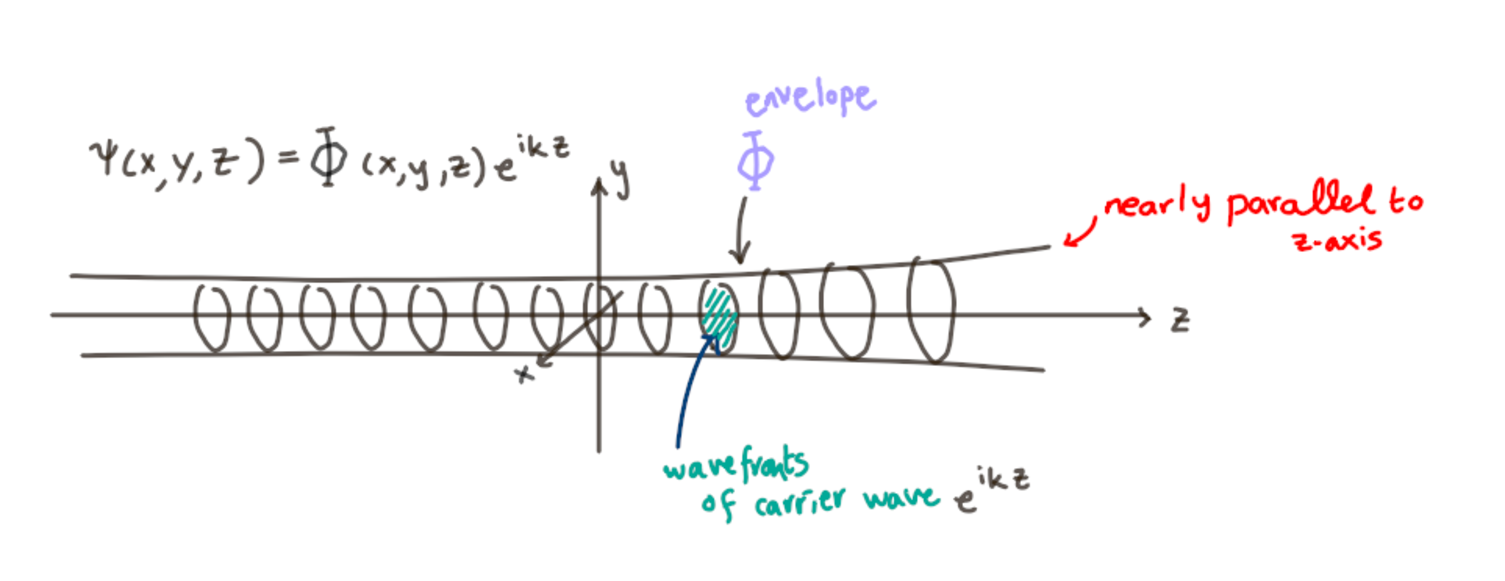
\includegraphics[width=0.6\linewidth]{paraxial_beam.pdf}
\captionof{figure}{cartoon of a paraxial wave-field $\psi_{\omega}(\vec{r})$ displaying beam propagation properties along the z-axis. The slowly varying complex envelope is modulated by a carrying plane wave.}
\end{Figure}
Note that the longitudinal variation of the complex envelope $\Delta z = \lambda = 2 \pi/k$ is required to be smaller than the complex envelope itself
\begin{equation}\label{eq:8}
\frac{\Delta \Phi(\vec{r})}{\Phi(\vec{r})} \leq 1
\end{equation}
using equation (\ref{eq:8}) and the longitudinal variation $\Delta z$  in the Helmholtz equation yields the paraxial Helmholtz equation in the vacuum
\begin{equation}\label{eq:9}
\left (\nabla_{T}^{2} + 2 i k \frac{\partial }{\partial z}\right ) \Phi(\vec{x , y, z}) = 0
\end{equation}

\subsubsection{Refractive index and the projection approximation}
In the presence of static, non-magnetic, scattering material media the complex scalar X-ray wave-field can still be studied by using the inhomogeneous Helmholtz equation 
\begin{equation}\label{eq:10}
\left ( k^2 n^2 (\vec{r}) + \nabla^{2}  \right )\Psi(\vec{r},t) = 0,
\end{equation}
where $n(\vec{r})$ is the position dependent and complex form for the refractive index, the real part of which corresponds to the refractive index and the imaginary part of this complexified refractive index can be related to the absorptive properties of a sample\cite{PagsTutes}.
\begin{equation}\label{eq:11}
n(x, y, z) = 1 - \delta(x, y, z) + i \beta(x, y, z),
\end{equation}
where $|\delta|, |\beta| << 1$. Using the complex refractive index in the inhomogeneous paraxial Helmholtz equation yields the \textit{projection approximation}, which is an expression that describes the phase shift and attenuation undergone by an X-ray wave moving across a sample
\begin{equation}\label{eq:12}
\Phi(x, y, z_0) = \mathrm{exp} \left ( -ik \int_{0}^{z_0}(\delta - i\beta)dz\right ) \Phi(x, y, 0)
\end{equation}
\begin{Figure}
\centering
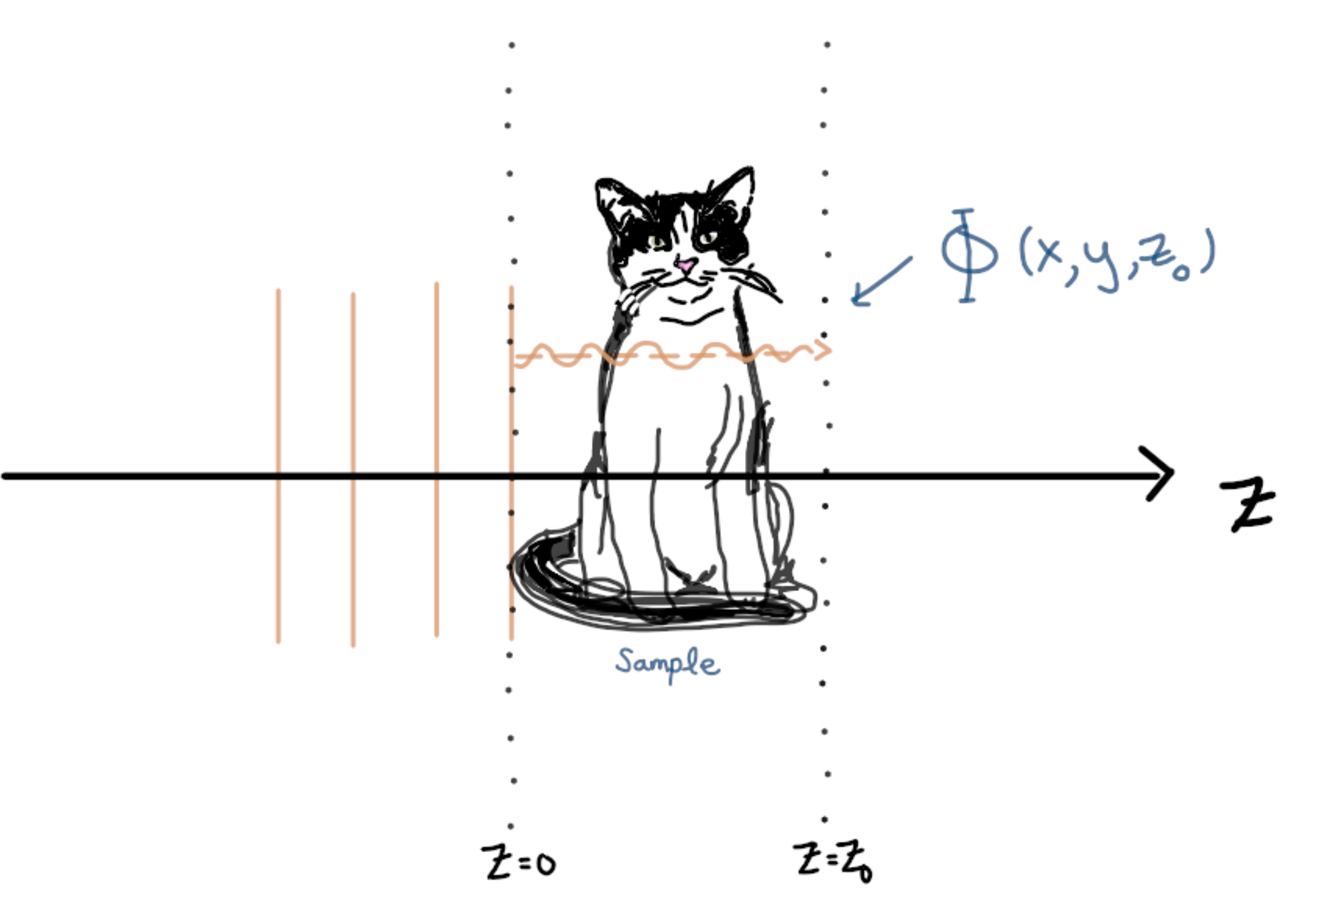
\includegraphics[width=0.6\linewidth]{projection_approximation.pdf}
\captionof{figure}{Schematic diagram of the projection approximation adapted from references \cite{CH49} and \cite{Pags2006}. The sample and is contained within the space between $z = 0$ and $z = z_0$. The sample is described by its refractive index $n(\vec{r})$ which differs from the the refractive index of the air volume that surrounds the sample.In this figure one can see that the path of X-rays passing through an object can be described by defining a surface immediately downstream from the irradiated object (i.e. $z = z_0$) at which the transferred transverse intensity and phase changes of the incident X-rays are imprinted\cite{CH49}. }
\end{Figure}
The projection approximation assumes that X-ray flow may be well approximated by straight lines parallel to z\cite{PagsTutes} and that most X-rays passing through an object do not actually interact with the sample material (i.e. minimal to no scattering occurs within the sample, a fair assumption due to small magnitude of the complex \textit{refractive index} of X-rays). Neglecting scattering effects is mathematically equivalent to discarding the transverse Laplacian term in equation (\ref{eq:9})\cite{CH49}, in addition X-ray--matter interaction must be taken into account in equation (\ref{eq:9}) making it the inhomogeneous paraxial Helmholtz equation
\begin{equation}\label{eq:13}
\left ( 2 i \frac{\partial }{\partial z} + k ( n^2 (x, y, z) - 1 )\right ) \Phi(\vec{x , y, z}) = 0.
\end{equation}

\subsubsection{Intensity and phase-shift}
Refraction is a property that may be augmented by the intensity attenuation due to the imaged object. This latter quantity may be obtained by taking the squared
modulus of equation (\ref{eq:12}), to give the \textit{Beer-Lambert law}\cite{PagsTutes}
\begin{equation}\label{eq:14}
I(x, y, z_0) = \mathrm{exp}[-\int_{t} \mu(x, y, z) dz] I(x, y, 0),
\end{equation}
where the expression above relates the imaginary part of the refractive index $\beta$ to the \textit{linear attenuation coefficient} $\mu = 2k\beta$.

Since we are working with a wave picture, refraction is associated with wave-front deformation rather than ray deflection, therefore the projection approximation term involving the refractive index $\delta$ (associated refractive properties of the object), quantifies the deformation of the X-ray wave-fronts due to passage through the sample object. Physically, for each fixed transverse coordinate $(x, y)$, phase-shifts (and the associated wave-front deformations) are continuously accumulated along energy-flow streamlines\cite{PagsTutes}.
\begin{equation}\label{eq:15}
\Delta \phi(x, y) = -k \int_{t}\delta(x, y, z)dz,
\end{equation}
where $k$ is the X-ray wave-number, $t$ is the projected thickness of the object in the direction of the beam propagation.

\subsubsection{Transport-of-intensity equation}
The transport-of-intensity equation (TIE) expresses the intensity and phase evolution of a paraxial monochromatic scalar electromagnetic or matter wave on propagation\cite{Pags2002}. The TIE is also used to quantify the contrast (i.e. refractive (phase) effects) present in propagation-based X-ray phase contrast images\cite{PagsTutes}.

More concisely, the TIE physically describes the divergence of the transverse energy-flow vector known as the Poynting vector $(\textbf{S})$. If the divergence of this vector is positive, (i.e. the wave-field is locally expanding), optical energy moves away from the local optic axis and so the longitudinal derivative of
intensity will be negative. The converse occurs if the divergence of the Poynting vector is negative, and so the longitudinal derivative of intensity will be positive\cite{PagsTutes}.
\begin{equation}\label{eq:16}
-\nabla_{T} [I(x, y, z) \nabla_{T} \phi(x, y, z)] = k \frac{\partial I (x, y, z)}{\partial z}.
\end{equation}
where $k$ is the wave-number, $I(x, y, z)$ is the intensity and $\phi(x, y, z)$ is the phase of the X-ray beam, the Poynting vector $\textbf{S} \propto I(x, y, z) \nabla_{T} \phi(x, y, z)$.

\section{Investigations}
The simulation that I am presently working on involves a cylinder made of a single material (i.e. monomorphic) with constant density. My supervisor and I are curious to see if we can verify a claim in one of the texts I am using in my research. This claim concerns a propagation based phase contrast imaging (PBI) algorithm that was first developed by Paganin et al. (2002)\cite{Pags2002}\cite{CH49}. Specifically, the claim states that the stability of Paganin's algorithm is thought to be dependent among other factors in the ratio between $\delta$ and $\mu$, both of which are proportional to the density of the medium. The conclusion from this claim is essentially that: any changes in material density throughout the material would not affect the imaging process. My supervisor suspects that this statement might not be entirely correct and we want to verify if the stability of the Paganin et al. (2002) algorithm is dependent instead on the ratio of the differences in the refraction and attenuation coefficients $\Delta \delta$ and $\Delta \mu$.

\subsubsection{Current progress}
I am inspiring some of my work in a paper by Beltran et al. (2010) (see reference \cite{Beltran}), their approach requires just a single phase-contrast projection, and enables the user to focus on a material of interest. In the case of my simulation, I set the complex refractive index, and thickness of the imaged cylinder based on the parameters given in Beltran et al.(2010)\cite{CH49}. For simplicity, my supervisor and I decided that I should break my simulation into simpler tasks. Therefore my first simulation will be that of a single monomorphic cylinder, and later on I will work on 2 cylinders, one embedded on another, both these cylinders will have different densities, since I want to understand how much density difference is needed before I see phase contrast in my simulation.
To solve the transport-of-intensity equation (TIE) and go beyond the projection approximation I have designed a differential equation solver using the fourth order Runge-Kutta algorithm. Since there is an intrinsic link between the phase and the TIE, I decided to solve re-write equation (\ref{eq:15}) in differential form and solve it simultaneously to the TIE in my code.
So far I have been able to recover the phase gained by the incident X-ray wave-fronts as they cross the cylindrical material I simulated.
\subsubsection{Results}
\begin{Figure}
\centering
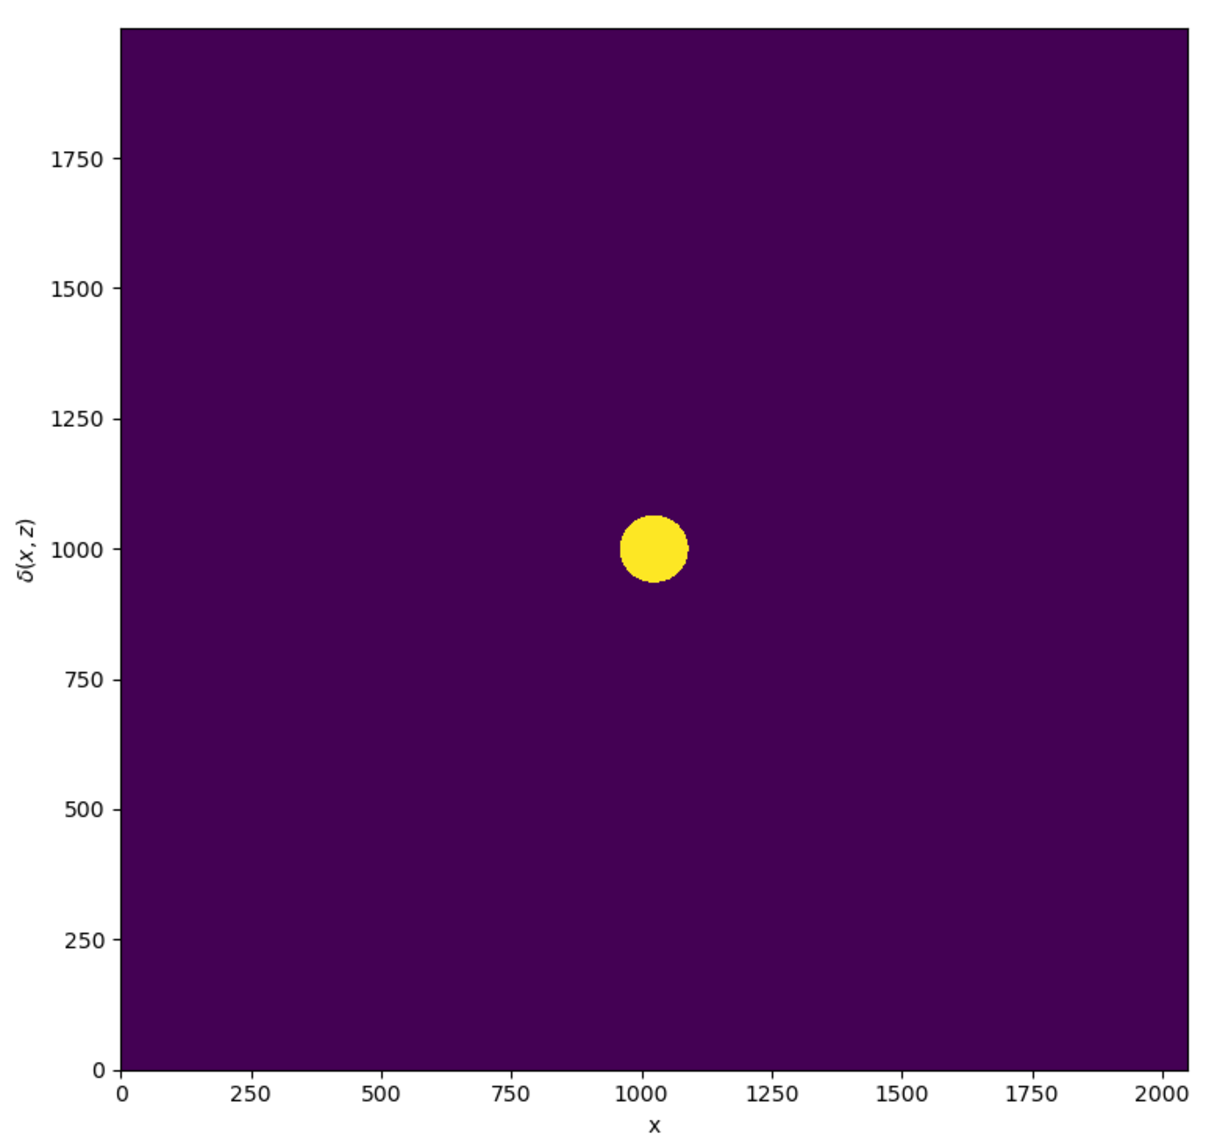
\includegraphics[width=0.6\linewidth]{cross_section.pdf}
\captionof{figure}{I made this 2D plot to verify that the cross-sectional are a of my simulated cylinder did indeed reflect the correct geometry. Here one can see a purple background representing the complex refractive index value of the vacuum $\delta = 0$ and that of the cylinder in yellow $\delta_0 = 462.8 \times 10^{-9}$ (as was reported in \cite{Beltran} for the PERSPEX sample).}
\end{Figure}
\begin{Figure}
\centering
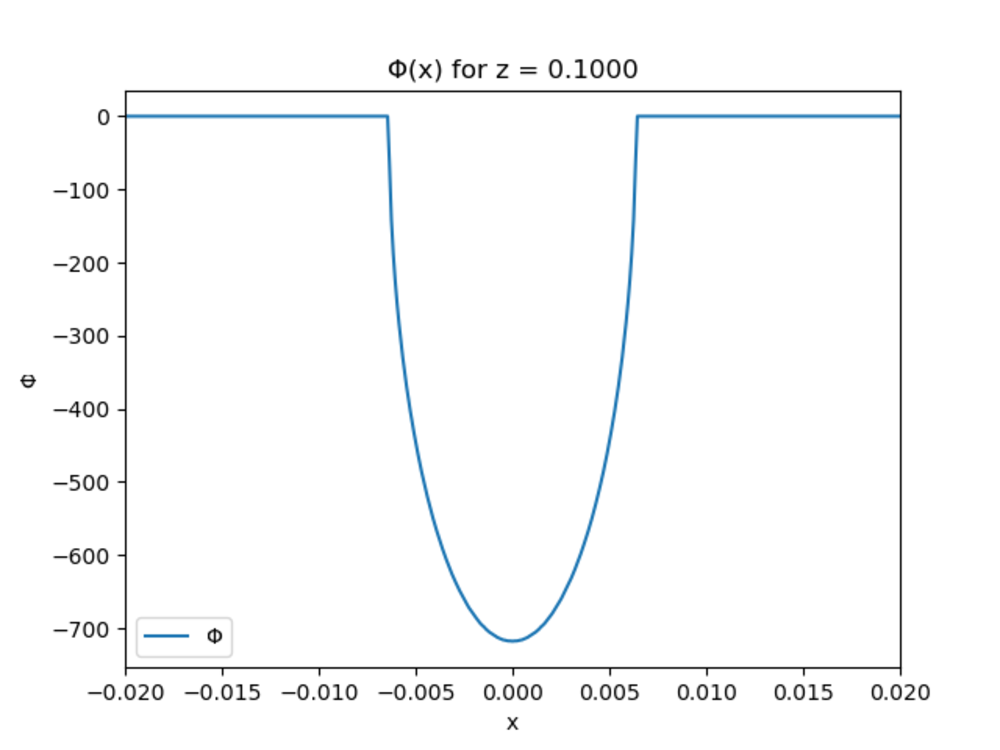
\includegraphics[width=0.6\linewidth]{20000.pdf}
\captionof{figure}{The position-dependent phase shift I discovered by using fourth order Runge-Kutta.}
\end{Figure}

\section{Future Plans}
I aim to finish my simulation by creating a graphic user interface (GUI) that allows the user to modify interactively the density parameters of the imaged concentric cylinders in the simulation. The goal is to make a easily operated visual representation of the changes in phase and intensity of the X-rays as they interact with the object in-situ.

In the foreseeable future my supervisor and I plan to diversify my project by making me do some simulations about a topic known as speckle analysis. A speckle pattern is commonly produced by interference of coherent light wave-fronts as these transmit through or reflect from a random phase assigning object (scattering medium), the process is known to encode information about the scattering medium that created the speckle\cite{Specks}. The main goal of making me do the speckle simulations is for me to understand the possible sources and causes of speckles in X-ray imaging, and to be able to decode speckle patterns.

% I also plan to aid my supervisor with testing a newly obtained silver target source of X-rays for his lab apparatus. I aim to do data analysis to compare the results from the new silver target to the classic tungsten target used in the apparatus currently.

\section{Conclusion}
The present aim of my project is to create simulation to investigate how the phase of incident X-rays changes as the density of a sample material in an arbitrary imaging system changes. My investigation will be extended by simulating two distinct materials under the same wave-field and see if and how distinctly phase contrast occurs. The eventual goal of this simulation is to verify if successful phase retrieval can be done of the imaged objects given their variable densities. In this report I present a brief outline of the theoretical perspective of coherent X-ray imaging, a description of my current progress and future aims.

\bibliography{mybib}
\bibliographystyle{unsrt}
\end{document}

% MAXWELL'S equations
% \begin{equation}
% \left ( \frac{1}{c^2} \frac{\partial^2 }{\partial t^2} -\nabla^2 \right )\mathbf{E}(\vec{r},t) = 0,
% \end{equation} 

% \begin{equation}
% \left ( \frac{1}{c^2} \frac{\partial^2 }{\partial t^2} -\nabla^2 \right )\mathbf{B}(\vec{r},t) = 0.
% \end{equation} 
